\documentclass[journal,12pt,twocolumn]{IEEEtran}

\usepackage{setspace}
\usepackage{gensymb}
\singlespacing
\usepackage[cmex10]{amsmath}

\usepackage{amsthm}

\usepackage{mathrsfs}
\usepackage{txfonts}
\usepackage{stfloats}
\usepackage{bm}
\usepackage{cite}
\usepackage{cases}
\usepackage{subfig}

\usepackage{longtable}
\usepackage{multirow}

\usepackage{enumitem}
\usepackage{mathtools}
\usepackage{steinmetz}
\usepackage{tikz}
\usepackage{circuitikz}
\usepackage{verbatim}
\usepackage{tfrupee}
\usepackage[breaklinks=true]{hyperref}
\usepackage{graphicx}
\usepackage{tkz-euclide}

\usetikzlibrary{calc,math}
\usepackage{listings}
    \usepackage{color}                                            %%
    \usepackage{array}                                            %%
    \usepackage{longtable}                                        %%
    \usepackage{calc}                                             %%
    \usepackage{multirow}                                         %%
    \usepackage{hhline}                                           %%
    \usepackage{ifthen}                                           %%
    \usepackage{lscape}     
\usepackage{multicol}
\usepackage{chngcntr}

\DeclareMathOperator*{\Res}{Res}

\renewcommand\thesection{\arabic{section}}
\renewcommand\thesubsection{\thesection.\arabic{subsection}}
\renewcommand\thesubsubsection{\thesubsection.\arabic{subsubsection}}

\renewcommand\thesectiondis{\arabic{section}}
\renewcommand\thesubsectiondis{\thesectiondis.\arabic{subsection}}
\renewcommand\thesubsubsectiondis{\thesubsectiondis.\arabic{sub subsection}}


\hyphenation{optical networks semiconduc-tor}
\def\inputGnumericTable{}                                 %%

\lstset{
%language=C,
frame=single, 
breaklines=true,
columns=fullflexible
}
\date{March 2021}

\begin{document}

\newcommand{\BEQA}{\begin{eqnarray}}
\newcommand{\EEQA}{\end{eqnarray}}
\newcommand{\define}{\stackrel{\triangle}{=}}
\bibliographystyle{IEEEtran}
\raggedbottom
\setlength{\parindent}{0pt}
\providecommand{\mbf}{\mathbf}
\providecommand{\pr}[1]{\ensuremath{\Pr\left(#1\right)}}
\providecommand{\qfunc}[1]{\ensuremath{Q\left(#1\right)}}
\providecommand{\fn}[1]{\ensuremath{f\left(#1\right)}}
\providecommand{\e}[1]{\ensuremath{E\left(#1\right)}}
\providecommand{\sbrak}[1]{\ensuremath{{}\left[#1\right]}}
\providecommand{\lsbrak}[1]{\ensuremath{{}\left[#1\right.}}
\providecommand{\rsbrak}[1]{\ensuremath{{}\left.#1\right]}}
\providecommand{\brak}[1]{\ensuremath{\left(#1\right)}}
\providecommand{\lbrak}[1]{\ensuremath{\left(#1\right.}}
\providecommand{\rbrak}[1]{\ensuremath{\left.#1\right)}}
\providecommand{\cbrak}[1]{\ensuremath{\left\{#1\right\}}}
\providecommand{\lcbrak}[1]{\ensuremath{\left\{#1\right.}}
\providecommand{\rcbrak}[1]{\ensuremath{\left.#1\right\}}}
\theoremstyle{remark}
\newtheorem{rem}{Remark}
\newcommand{\sgn}{\mathop{\mathrm{sgn}}}
\providecommand{\abs}[1]{\vert#1\vert}
\providecommand{\res}[1]{\Res\displaylimits_{#1}} 
\providecommand{\norm}[1]{\lVert#1\rVert}
%\providecommand{\norm}[1]{\lVert#1\rVert}
\providecommand{\mtx}[1]{\mathbf{#1}}
\providecommand{\mean}[1]{E[ #1 ]}
\providecommand{\fourier}{\overset{\mathcal{F}}{ \rightleftharpoons}}
%\providecommand{\hilbert}{\overset{\mathcal{H}}{ \rightleftharpoons}}
\providecommand{\system}{\overset{\mathcal{H}}{ \longleftrightarrow}}
	%\newcommand{\solution}[2]{\textbf{Solution:}{#1}}
\newcommand{\solution}{\noindent \textbf{Solution: }}
\newcommand{\cosec}{\,\text{cosec}\,}
\providecommand{\dec}[2]{\ensuremath{\overset{#1}{\underset{#2}{\gtrless}}}}
\newcommand{\myvec}[1]{\ensuremath{\begin{pmatrix}#1\end{pmatrix}}}
\newcommand{\mydet}[1]{\ensuremath{\begin{vmatrix}#1\end{vmatrix}}}
\numberwithin{equation}{subsection}
\makeatletter
\@addtoreset{figure}{problem}
\makeatother
\let\StandardTheFigure\thefigure
\let\vec\mathbf
\renewcommand{\thefigure}{\theproblem}
\def\putbox#1#2#3{\makebox[0in][l]{\makebox[#1][l]{}\raisebox{\baselineskip}[0in][0in]{\raisebox{#2}[0in][0in]{#3}}}}
     \def\rightbox#1{\makebox[0in][r]{#1}}
     \def\centbox#1{\makebox[0in]{#1}}
     \def\topbox#1{\raisebox{-\baselineskip}[0in][0in]{#1}}
     \def\midbox#1{\raisebox{-0.5\baselineskip}[0in][0in]{#1}}
\vspace{3cm}
\title{ASSIGNMENT 2}
\author{MANIKANTA VALLEPU - AI20BTECH11014}
\maketitle
\newpage
\bigskip
\renewcommand{\thefigure}{\theenumi}
\renewcommand{\thetable}{\theenumi}
Download all python codes from 
\begin{lstlisting}
https://github.com/manik2255/AI1103-PROBABILITY-AND-RANDOM-VARIABLES/blob/main/ASSIGNMENT_2/ASSIGNMENT_2_GRAPH.py
\end{lstlisting}
%
and latex-tikz codes from 
%
\begin{lstlisting}
https://github.com/manik2255/AI1103-PROBABILITY-AND-RANDOM-VARIABLES/blob/main/ASSIGNMENT_2/ASSIGNMENT_2.tex
\end{lstlisting}
\section{Problem.GATE.14}
A continuous random variable $X$ has a probability density function 
$\fn{x} = e^{-x}$,$0<x<\infty$. Then $P(X > 1)$ is

\section{Solution}
Given,
\begin{align} \label{1}
\fn{x} = e^{-x} , 0<x<\infty
\end{align}
We have to find \pr{X>1},
\begin{align}
\pr{X>1} = \int_{1}^{\infty}{\fn{x}}\,dx\label{2}
\end{align}
Using \eqref{1} in \eqref{2}
\begin{align}
\pr{X>1} &= \int_{1}^{\infty}{e^{-x}}\,dx\\
&= \left[-e^{-x}\right]_1^{\infty}\\
&= (-e^{-\infty}) - (-e^{-1})\\
&= e^{-1}\\
&= \frac{1}{e}\\
 \implies \pr{X>1} &= 0.368
\end{align}
Finding the probability using uniform distribution,

Let $F_X(x)$ be the cumulative distribution function of random variable X.
\begin{align}
    F_X(x)=\int_{0}^x \fn{x} dx\label{x}
\end{align}
$F_X(x)$ can be obtained from the uniform distribution of a random variable U on (0,1) and let U=$e^{-x}$. 
\begin{align}
    0 < U < 1
\end{align}
As for random variable X also,
\begin{align}
    0 < F_X(x) < 1
\end{align}
This similarity between U and $F_X(x)$ is used to generate the random variable X from U.
\begin{align}
    F_X(x)&=\pr{X<x}\\
    &=\pr{-\log_e U<x}\\
    &=\pr{U<e^{-x}}\\
    &=F_U(e^{-x})\label{y}
\end{align}
From uniform distribution,
\begin{align}
    F_U(x)= x ,0<x<1 \label{z}
\end{align}
\begin{figure}[htp]
    \centering
    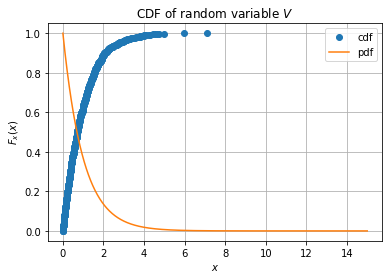
\includegraphics[width=\columnwidth]{Figure.png}
\end{figure}
\\Using \eqref{z} in \eqref{y},
\\Cumulative distribution function (CDF) of random variable X is,
\begin{align}
F_X(x) &= \pr{X<x}\\
&= 1 -e^{-x} ,0<x<\infty \label{g}
\end{align}
Now we have to find \pr{X>1},
\begin{align}
    \pr{X>1} &= 1-\pr{X<1}
\end{align}
Using  \eqref{g},
\begin{align}
    \pr{X>1} &= 1-(1 -e^{-1})\\
    \pr{X>1} &= e^{-1}\\
   \implies \pr{X>1} &= 0.368 
\end{align}

\end{document}
